\documentclass{article}
\usepackage[utf8]{vietnam}
\usepackage[utf8]{inputenc}
\usepackage{anyfontsize,fontsize}
\changefontsize[13pt]{13pt}
\usepackage{commath}
\usepackage[d]{esvect}
\usepackage{parskip}
\usepackage{xcolor}
\usepackage{amssymb}
\usepackage{slashed,cancel}
\usepackage{indentfirst}
\usepackage{pdfpages}
\usepackage{graphicx}
\usepackage{upgreek}
\usepackage{nccmath,nicematrix}
\usepackage{mathtools}
\usepackage{amsfonts}
\usepackage{amsmath,systeme}
\usepackage[thinc]{esdiff}
\usepackage{hyperref}
\usepackage{bm,physics}
\usepackage{fancyhdr}
\usepackage{tikz-feynman}
%footnote
\pagestyle{fancy}
\renewcommand{\headrulewidth}{0pt}%
\fancyhf{}%
\fancyfoot[L]{Vật lý Lý thuyết}%
\fancyfoot[C]{\hspace{6.5cm} \thepage}%


\usepackage{geometry}
\geometry{
	a4paper,
	total={170mm,257mm},
	left=20mm,
	top=20mm,
}


\newcommand{\image}[1]{
	\begin{figure}[H]
		\centering
		\includegraphics[width=8.0cm,height=5.0cm]{pic/#1}
		\label{#1}
	\end{figure}
}
\renewcommand{\l}{\ell}
\newcommand{\dps}{\displaystyle}
\newcommand{\mean}[1]{\langle{#1}\rangle}
\newcommand{\at}[2]{\bigg\rvert_{#1}^{#2} }


\renewcommand{\baselinestretch}{2.0}


\title{\Huge{}}

\hypersetup{
	colorlinks=true,
	linkcolor=black,
	filecolor=magenta,      
	urlcolor=cyan,
	pdftitle={},
	pdfpagemode=FullScreen,
}

\urlstyle{same}

\begin{document}
\setlength{\parindent}{20pt}
\newpage
\author{TRẦN KHÔI NGUYÊN \\ VẬT LÝ LÝ THUYẾT}
\maketitle
%\tableofcontents

%\section{Định lý Bloch}
%Hàm riêng của Hamiltonian một điện tử
%\begin{gather}
%	H_{\text{1e}} = -\frac{\hbar^{2} \nabla^{2}}{2m} + V_{0}(\mathbf{r}),
%\end{gather}
%với $V_{0}(\mathbf{r})$ là thế tuần hoàn $V_{0}(\mathbf{r} + \mathbf{R}) = V_{0}(\mathbf{r})$, hàm Bloch có dạng
%\begin{gather}
%	\psi_{\lambda \mathbf{k}}(\mathbf{r}) = e^{i \mathbf{k} \cdot \mathbf{r}} u_{\lambda \mathbf{k}}(\mathbf{r}),
%\end{gather}
%trong đó $u_{\lambda \mathbf{k}}(\mathbf{r} + \mathbf{R}) = u_{\lambda \mathbf{k}}(\mathbf{r})$.

\section{Hamiltonian lượng tử hoá lần 2}
\subsection{Hamiltonian tương tác với ánh sáng}
Hamiltonian hệ điện tử trong tinh thể tương tác với trường ngoài(ánh sáng), khi chưa có xét đến tương tác điện tử $-$ điện tử là
\begin{gather}
	H = \sum_{i} = H_{\text{1e}} (\mathbf{r}_{i}, t) = \sum_{i} H_{\text{1e}}^{0}(\mathbf{r}_{i}) + \sum_{i} H_{1e}^{e-L} (\mathbf{r}_{i}, t).
\end{gather}
Hamiltonian lượng tử hoá lần 2 trong hệ cơ sở trực chuẩn $\left\{ \ket{\psi_{\lambda \mathbf{k}}} \right\}$
\begin{gather}
	\braket{\psi_{\lambda \mathbf{k}}}{\psi_{\lambda' \mathbf{k}'}} = \delta_{\lambda, \lambda'} \delta_{\mathbf{k}, \mathbf{k}'},
\end{gather}
trong đó $\lambda$ là chỉ số dải với vector sóng $\mathbf{k}$, và Hamiltonian có dạng
\begin{gather}
	H = H^{0} + H^{e-L},
\end{gather}
trong đó
\begin{gather}
	H^{0} = \sum_{\lambda \lambda' \mathbf{k} \mathbf{k}'} = \bra{\psi_{\lambda \mathbf{k}}} H_{\text{1e}}^{0} \ket{\psi_{\lambda' \mathbf{k}'}} a^{\dagger}_{\lambda \mathbf{k}} a_{\lambda' \mathbf{k}'},\\
	H^{e-L} = \sum_{\lambda \lambda' \mathbf{k} \mathbf{k}'} \bra{\psi_{\lambda \mathbf{k}}} H_{1e}^{e-L} (\mathbf{r} , t) \ket{\psi_{\lambda' \mathbf{k}'}} a^{\dagger}_{\lambda \mathbf{k}} a_{\lambda' \mathbf{k}'},
	\label{Hamiltonian e-L}
\end{gather}
trong đó các toán tử sinh huỷ tuân theo hệ thức phản giao hoán
\begin{gather}
	\{a_{\lambda \mathbf{k}}, a^{\dagger}_{\lambda \mathbf{k}'}\} = a_{\lambda \mathbf{k}} a^{\dagger}_{\lambda' \mathbf{k}'} + a^{\dagger}_{\lambda' \mathbf{k}'} a_{\lambda \mathbf{k}}  = \delta_{\lambda, \lambda'} \delta_{\mathbf{k}, \mathbf{k}'}
	\label{eq: anti commutators 1},\\
	\left\{a_{\lambda \mathbf{k}}, \mathbf{a}_{\lambda' \mathbf{k}'}  \right\} =
	\{a^{\dagger}_{\lambda \mathbf{k}}, a^{\dagger}_{\lambda' \mathbf{k}'}  \} = 0.
	\label{eq: anti commutators 2}
\end{gather}
Nếu chọn hệ cơ sở là hàm riêng của $H_{\text{1e}}^{0}$, tức là
\begin{gather}
	H^{0} \psi_{\lambda \mathbf{k}} = \mathcal{E}_{\lambda}(\mathbf{k}) \psi_{\lambda \mathbf{k}},
\end{gather}
thì $H^{0}$ trở thành
\begin{gather}
	H^{0} = \sum_{\lambda \mathbf{k}} \mathcal{E}_{\lambda} a_{\lambda \mathbf{k}}^{\dagger} a_{\lambda \mathbf{k}}.
\end{gather}
\subsubsection*{$\mathbf{H^{e-L}}$ trong gauge vận tốc}
Sử dụng gauge vận tốc, các yếu tố ma trận tương tác giữa điện tử $-$ ánh sáng là
\begin{equation}
	\begin{aligned}
		\bra{\psi_{\lambda \mathbf{k}}} H_{\text{1e}}^{e - L}(\mathbf{r}, t) \ket{\psi_{\lambda' \mathbf{k}'}} & = \bra{\psi_{\lambda \mathbf{k}}} \frac{e}{m} \mathbf{A}(\mathbf{r}, t) \cdot \mathbf{p} \ket{\psi_{\lambda' \mathbf{k}'}} + \frac{e^{2} A^{2}}{2m} \delta_{\lambda, \lambda'} \delta_{\mathbf{k}, \mathbf{k}'} \\
		                                                                                                       & \approx \frac{e}{m} \mathbf{A}(t) \cdot \bra{\psi_{\lambda \mathbf{k}}} \mathbf{p} \ket{\psi_{\lambda' \mathbf{k}'}} + \frac{e^{2} A^{2}}{2m} \delta_{\lambda, \lambda'} \delta_{\mathbf{k}, \mathbf{k}'},
	\end{aligned}
	\label{eq:H e-L VG}
\end{equation}
trong đó yếu tố ma trận xung lượng được khai triển qua hàm Bloch như sau
\begin{equation}
	\begin{aligned}
		\bra{\psi_{\lambda \mathbf{k}}} \mathbf{p} \ket{\psi_{\lambda' \mathbf{k}'}}
		 & = \int \frac{d^{3} r}{V} u_{\lambda \mathbf{k}}^{*} e^{-i \mathbf{k} \cdot \mathbf{r}} \mathbf{p} e^{i \mathbf{k}' \cdot \mathbf{r}} u_{\lambda' \mathbf{k}'}(\mathbf{r})                                                                                                                              \\
		 & = \frac{1}{N} \sum_{i}^{N} e^{i (\mathbf{k} - \mathbf{k}') \cdot \mathbf{R}_{i}} \int_{V_{\text{cell}}} \frac{d^{3} r}{V_{\text{cell}}} u_{\lambda \mathbf{k}}^{*} (\mathbf{r}) e^{-i \mathbf{k} \cdot \mathbf{r}} \mathbf{p} e^{i \mathbf{k}' \cdot \mathbf{r}} u_{\lambda' \mathbf{k}'}(\mathbf{r}),
	\end{aligned}
\end{equation}
mà ta có $\dps\sum_{i}^{N} e^{i (\mathbf{k}' - \mathbf{k}) \cdot \mathbf{R}_{i}} = N \delta_{\mathbf{k}, \mathbf{k}'}$, ta thu được
\begin{equation}
	\begin{aligned}
		\bra{\psi_{\lambda \mathbf{k}}} \mathbf{p} \ket{\psi_{\lambda' \mathbf{k}'}}
		 & = \int_{V_{\text{cell}}} \frac{d^{3} r}{V_{\text{cell}}} u_{\lambda \mathbf{k}}^{*} (\mathbf{r}) e^{-i \mathbf{k} \cdot \mathbf{r}} \mathbf{p} e^{i \mathbf{k}' \cdot \mathbf{r}} u_{\lambda' \mathbf{k}'}(\mathbf{r}) \\
		 & = \mathbf{p}_{\lambda \lambda'}(\mathbf{k}) \delta_{\mathbf{k}, \mathbf{k}'} \equiv \bra{u_{\lambda \mathbf{k}}} \mathbf{p}(\mathbf{k}) \ket{u_{\lambda' \mathbf{k}}},
	\end{aligned}
	\label{eq: matrix momentum}
\end{equation}
trong đó
\begin{gather}
	\mathbf{p}(\mathbf{k}) = e^{-i \mathbf{k} \cdot \mathbf{r}} \mathbf{p} e^{i \mathbf{k} \cdot \mathbf{r}}.
\end{gather}
Ta biểu diễn Hamiltonian 1 hạt trong không gian $k$
\begin{gather}
	H_{\text{1e}}^{0}(\mathbf{k}) = e^{-i \mathbf{k} \cdot \mathbf{r}} H_{\text{1e}}^{0} e^{i\mathbf{k} \cdot \mathbf{r}},
\end{gather}
lấy đạo hàm theo $k$ cho phương trình (16), ta có
\begin{equation}
	\begin{aligned}
		\nabla_{\mathbf{k}} H_{1e}^{0}(\mathbf{k})
		 & = -i \mathbf{r} e^{- i \mathbf{k} \cdot \mathbf{r}} H_{1e} e^{i \mathbf{k} \cdot \mathbf{r}} + e^{-i \mathbf{k} \cdot \mathbf{r}} H_{1e}^{0} i \mathbf{r} e^{i \mathbf{k} \cdot \mathbf{r}} \\
		 & = i e^{-i \mathbf{k} \cdot \mathbf{r}}\left(  H_{1e}^{0}\mathbf{r}  - \mathbf{r} H_{1e}^{0} \right) e^{i \mathbf{k} \cdot \mathbf{r}}                                                       \\
		 & = i e^{-i \mathbf{k} \cdot \mathbf{r}} [H_{1e}^{0}, \mathbf{r}] e^{i \mathbf{k} \cdot \mathbf{r}}                                                                                           \\
		 & = i [H_{1e}^{0}(\mathbf{k}), \mathbf{r}].
	\end{aligned}
\end{equation}
Lại có hệ thức giao hoán giữa $[H_{\text{1e}}^{0}, \mathbf{r}] $
\begin{align}
	[H_{\text{1e}}^{0}, \mathbf{r}]
	                                                                                                                     & = -\frac{i\hbar}{m} \mathbf{p} \nonumber                                                                                    \\
	\Leftrightarrow e^{-i \mathbf{k} \cdot \mathbf{r}} [H_{\text{1e}}^{0}, \mathbf{r}] e^{i \mathbf{k} \cdot \mathbf{r}} & = e^{-i \mathbf{k} \cdot \mathbf{r}} \left(- \frac{i\hbar}{m} \mathbf{p}\right) e^{i \mathbf{k} \cdot \mathbf{r}} \nonumber \\
	\Leftrightarrow \nabla_{\mathbf{k}} H_{1e}^{0}(\mathbf{k})                                                           & = \frac{\hbar}{m} \mathbf{p}(\mathbf{k}) \nonumber                                                                          \\
	\Leftrightarrow \mathbf{p}(\mathbf{k})                                                                               & = \frac{m}{\hbar} \nabla_{\mathbf{k}} H_{1e}^{0}(\mathbf{k}).
\end{align}
Các yếu tố ma trận xung lượng từ phương trình \eqref{eq: matrix momentum} có thể tính được thông qua
\begin{gather}
	\mathbf{p}_{\lambda \lambda'} (\mathbf{k}) = \frac{m}{\hbar} \bra{u_{\lambda \mathbf{k}}} \nabla_{\mathbf{k}} H_{1e}^{0}(\mathbf{k}) \ket{u_{\lambda' \mathbf{k}'}}.
\end{gather}
Từ phương trình \eqref{eq:H e-L VG}, Hamiltonian tương tác điện tử và ánh sáng ở lượng tử hoá lần 2 trong gauge vận tốc có dạng
\begin{gather}
	H^{e - L} = \frac{e}{m} \mathbf{A}(t) \cdot \sum_{\lambda \lambda' \mathbf{k}} \mathbf{p}_{\lambda \lambda'}(\mathbf{k}) a_{\lambda \mathbf{k}}^{\dagger} a_{\lambda' \mathbf{k}} + \frac{e^{2} A^{2}}{2m} \sum_{\lambda \mathbf{k}} a_{\lambda \mathbf{k}}^{\dagger} a_{\lambda \mathbf{k}}.
	\label{eq: H e-L VG 2nd quantization}
\end{gather}
\subsubsection*{$\mathbf{H^{e-L}}$ trong gauge độ dài}
Trong gauge độ dài, Hamiltonian tương tác điện tử $-$ ánh sáng \eqref{Hamiltonian e-L} là
\begin{gather}
	\bra{\psi_{\lambda \mathbf{k}}} H_{1e}^{e-L}(\mathbf{r}, t) \ket{\psi_{\lambda' \mathbf{k}'}} = \bra{\psi_{\lambda \mathbf{k}}} e \mathbf{E}(\mathbf{r}, t) \cdot \mathbf{r} \ket{\psi_{\lambda' \mathbf{k}'}} \simeq e \mathbf{E}(t) \cdot \bra{\psi_{\lambda \mathbf{k}}} \mathbf{r} \ket{\psi_{\lambda' \mathbf{k}'}},
\end{gather}
trong đó yếu tố ma trận vị trí được cho bởi
\begin{equation}
	\begin{aligned}
		\bra{\psi_{\lambda \mathbf{k}}} \mathbf{r} \ket{\psi_{\lambda' \mathbf{k}'}}
		 & = \int \frac{d^{3} r}{V} u_{\lambda \mathbf{k}}^{*}(\mathbf{r}) e^{-i \mathbf{k} \cdot \mathbf{r}} \mathbf{r} e^{i \mathbf{k}' \cdot \mathbf{r}} u_{\lambda' \mathbf{k}'}(\mathbf{r})                                                                                                                                  \\
		 & = i \nabla_{\mathbf{k}} \left( \int \frac{d^{3} r}{V} u_{\lambda \mathbf{k}}^{*} (\mathbf{r}) e^{-i \mathbf{k} \cdot \mathbf{r}} e^{i \mathbf{k}' \cdot \mathbf{r}} u_{\lambda' \mathbf{k}'}(\mathbf{r}) \right)                                                                                                       \\
		 & \quad - i \int \frac{d^{3} r}{V} \left( \nabla_{\mathbf{k}} u_{\lambda \mathbf{k}}^{*}(\mathbf{r}) \right) e^{i \mathbf{k} \cdot \mathbf{r}} e^{i \mathbf{k}' \cdot \mathbf{r}} u_{\lambda' \mathbf{k}'}(\mathbf{r})                                                                                                   \\
		 & = i \nabla_{\mathbf{k}} \left( \frac{1}{N} \sum_{i}^{N} e^{-i \left(\mathbf{k} - \mathbf{k}'\right) \cdot \mathbf{R}_{i}} \int_{V_{\text{cell}}} \frac{d^{3} r}{V_{\text{cell}}} u_{\lambda \mathbf{k}}^{*}(\mathbf{r}) e^{-i (\mathbf{k} - \mathbf{k}') \cdot \mathbf{r}} u_{\lambda' \mathbf{k}'}(\mathbf{r})\right) \\
		 & \quad - i \frac{1}{N} \sum_{i}^{N} e^{-i (\mathbf{k} - \mathbf{k}') \cdot \mathbf{R}_{i}} \int_{V_{\text{cell}}} \frac{d^{3}r}{V_{\text{cell}}} ( \nabla_{\mathbf{k}} u_{\lambda \mathbf{k}}^{*}(\mathbf{r}) ) e^{-i (\mathbf{k} - \mathbf{k}') \cdot \mathbf{r}} u_{\lambda' \mathbf{k}'}(\mathbf{r}).
	\end{aligned}
\end{equation}
Áp dụng gần đúng sóng dài $k, k' \llless \frac{2\pi}{a}$, ta được
\begin{equation}
	\begin{aligned}
		\bra{\psi_{\lambda \mathbf{k}}} \mathbf{r} \ket{\psi_{\lambda' \mathbf{k}'}}
		 & \simeq i \nabla_{\mathbf{k}} \delta_{\mathbf{k}, \mathbf{k}'} \int_{V_{\text{cell}}} \frac{d^{3} r}{V_{\text{cell}}} \nabla_{\mathbf{k}} u_{\lambda \mathbf{k}}^{*}(\mathbf{r}) u_{\lambda' \mathbf{k}'}(\mathbf{r}) \\
		 & \quad - i \delta_{\mathbf{k}, \mathbf{k}'} \int_{V_{\text{cell}}} \frac{d^{3} r}{V_{\text{cell}}} (\nabla_{\mathbf{k}} u_{\lambda \mathbf{k}}^{*}(\mathbf{r})) u_{\lambda' \mathbf{k}'}(\mathbf{r})                  \\
		 & = i \nabla_{\mathbf{k}} \delta_{\mathbf{k}, \mathbf{k}'} \delta_{\lambda, \lambda'} - i \delta_{\lambda, \lambda'} \braket{\nabla_{\mathbf{k}} u_{\lambda \mathbf{k}}}{u_{\lambda' \mathbf{k}'}}.
		\label{eq: position matrix elements}
	\end{aligned}
\end{equation}
Ta định nghĩa yếu tố ma trận lưỡng cực như sau
\begin{gather}
	\boldsymbol{\xi}_{\lambda \lambda'}(\mathbf{k}) = - i \braket{\nabla_{\mathbf{k}} u_{\lambda \mathbf{k}}},
\end{gather}
như vậy các yếu tố ma trận vị trí ở phương trình \eqref{eq: position matrix elements} được viết lại dưới dạng
\begin{gather}
	\bra{\psi_{\lambda \mathbf{k}}} \mathbf{r} \ket{\psi_{\lambda' \mathbf{k}'}} = ( \boldsymbol{\xi}_{\lambda \lambda'}(\mathbf{k}) + i \delta_{\lambda \lambda'}\nabla_{\mathbf{k}} ) \delta_{\mathbf{k}, \mathbf{k}'}.
\end{gather}
Trong trường hợp $\lambda \neq \lambda'$, từ hệ thức giao hoán $[H_{\text{1e}}^{0}, \mathbf{r}]= -\frac{i\hbar}{m} \mathbf{p}$ và $\bra{\psi_{\lambda \mathbf{k}}} \mathbf{p} \ket{\psi_{\lambda' \mathbf{k}'}} = \mathbf{p}_{\lambda \lambda'}(\mathbf{k}) \delta_{\mathbf{k}, \mathbf{k}'}$, ta có
\begin{equation}
	\begin{aligned}
		\mathbf{p}                                                                                                                                      & = \frac{im}{\hbar} [H_{\text{1e}}^{0}, \mathbf{r}]                                                                                                                               \\
		\quad \Leftrightarrow \bra{\psi_{\lambda \mathbf{k}}} \mathbf{p} \ket{\psi_{\lambda' \mathbf{k}'}}                                              & = \frac{im}{\hbar} \bra{\psi_{\lambda \mathbf{k}}} [H_{\text{1e}}^{0}, \mathbf{r}] \ket{\psi_{\lambda' \mathbf{k}'}}                                                             \\
		\Leftrightarrow -\frac{i \hbar}{m} \mathbf{p}_{\lambda \lambda'}(\mathbf{k})\delta_{\mathbf{k}, \mathbf{k}'}                                    & = \bra{\psi_{\lambda \mathbf{k}}} H_{1e}^{0} \mathbf{r} - \mathbf{r} H_{1e}^{0} \ket{\psi_{\lambda' \mathbf{k}'}}                                                                \\
		\Leftrightarrow -\frac{i \hbar}{m} \mathbf{p}_{\lambda \lambda'}                                                                                & =  (\mathcal{E}_{\lambda}(\mathbf{k}) - \mathcal{E}_{\lambda'}(\mathbf{k})) \bra{\psi_{\lambda \mathbf{k}}} \mathbf{r} \ket{\psi_{\lambda' \mathbf{k}'}}                         \\
		\Leftrightarrow -\frac{i \hbar}{m} \mathbf{p}_{\lambda \lambda'}                                                                                & =  (\mathcal{E}_{\lambda}(\mathbf{k}) - \mathcal{E}_{\lambda'}(\mathbf{k})) ( \boldsymbol{\xi}_{\lambda \lambda'}(\mathbf{k}) + i \delta_{\lambda \lambda'}\nabla_{\mathbf{k}} ) \\
		\Leftrightarrow -\frac{i \hbar}{m} \frac{\mathbf{p}_{\lambda \lambda'}}{\mathcal{E}_{\lambda}(\mathbf{k}) - \mathcal{E}_{\lambda'}(\mathbf{k})} & =  \boldsymbol{\xi}_{\lambda \lambda'}(\mathbf{k}).
	\end{aligned}
\end{equation}
Hamiltonian lượng tử hoá lần thứ 2 cho tương tác điện tử $-$ ánh sáng trong gauge độ dài
\begin{gather}
	H^{e-L} = e \mathbf{E}(t) \cdot \sum_{\lambda \lambda' \mathbf{k}} \boldsymbol{\xi}_{\lambda \lambda'}(\mathbf{k}) a_{\lambda \mathbf{k}}^{\dagger} a_{\lambda' \mathbf{k}} + i e \mathbf{E}(t) \cdot \sum_{\lambda \mathbf{k} \mathbf{k}'} \nabla_{\mathbf{k}} \delta_{\mathbf{k}, \mathbf{k}'} a_{\lambda \mathbf{k}}^{\dagger} a_{\lambda \mathbf{k}'},
	\label{eq: H e-L LG 2nd quantization}
\end{gather}
\subsection{Toán tử mật độ điện tích}
Toán tử mật độ điện tích được định nghĩa là
\begin{gather}
	\hat{\rho}_{\lambda' \lambda} (\mathbf{k}) = - \frac{\abs{e}}{V} \sum_{\mathbf{k}} a_{\lambda \mathbf{k}}^{\dagger} a_{\lambda \mathbf{k}}.
\end{gather}
ta cần khảo sát sự thay đổi của giá trị trung bình của toán tử mật độ điện tích theo thời gian
\begin{gather}
	\langle \rho_{\lambda' \lambda} \rangle = -\frac{\abs{e}}{V} \sum_{\mathbf{k}} \langle a_{\lambda \mathbf{k}}^{\dagger} a_{\lambda' \mathbf{k}} \rangle.
	\label{eq: operator charge density}
\end{gather}
Vậy, ma trận mật độ điện tích rút gọn có thể viết lại dưới dạng
\begin{gather}
	\rho_{\lambda' \lambda}(\mathbf{k}) = \langle a_{\lambda \mathbf{k}}^{\dagger} a_{\lambda' \mathbf{k}} \rangle.
	\label{eq: operator charge density matrix elements reduced}
\end{gather}
Để khảo sát phương trình \eqref{eq: operator charge density}, ta cần khảo sát $a_{\lambda \mathbf{k}}^{\dagger} a_{\lambda' \mathbf{k}}$ trong bức tranh Heisenberg.
\subsection{Phương trình chuyển động}
Phương trình chuyển động Heisenberg cho toán tử $a_{\lambda \mathbf{k}}^{\dagger} a_{\lambda' \mathbf{k}}$
\begin{gather}
	\frac{d}{dt} a_{\lambda \mathbf{k}}^{\dagger} a_{\lambda' \mathbf{k}} = \frac{i}{\hbar} [H, a_{\lambda \mathbf{k}}^{\dagger} a_{\lambda' \mathbf{k}}] + \cancelto{0}{\frac{\partial}{\partial t}a_{\lambda \mathbf{k}}^{\dagger} a_{\lambda' \mathbf{k}}},
	\label{eq: equation of motion}
\end{gather}
trong đó
\begin{equation}
	\begin{aligned}
		H & = H^{0} + H^{e-L}                                                                                                                                                                                                                                                                                                                                                                             \\
		  & = \sum_{\lambda \mathbf{k}} \mathcal{E}_{\lambda} a_{\lambda \mathbf{k}}^{\dagger} a_{\lambda \mathbf{k}} + \frac{e}{m} \mathbf{A}(t) \cdot \sum_{\lambda \lambda' \mathbf{k}} \mathbf{p}_{\lambda \lambda'}(\mathbf{k}) a_{\lambda \mathbf{k}}^{\dagger} a_{\lambda' \mathbf{k}} + \frac{e^{2} A^{2}}{2m} \sum_{\lambda \mathbf{k}} a_{\lambda \mathbf{k}}^{\dagger} a_{\lambda \mathbf{k}}.
	\end{aligned}
\end{equation}
Tính các giao hoán tử
\begin{equation}
	\begin{aligned}
		[H^{0},a_{\lambda \mathbf{k}}^{\dagger} a_{\lambda' \mathbf{k}}]
		 & = \sum_{\nu \mathbf{k'}} \mathcal{E}_{\nu}(\mathbf{k}') [a_{\nu \mathbf{k}'}^{\dagger} a_{\nu \mathbf{k}'}, a_{\lambda \mathbf{k}}^{\dagger} a_{\lambda' \mathbf{k}}]                                                                                                                                                          \\
		 & = \sum_{\nu \mathbf{k'}} \mathcal{E}_{\nu}(\mathbf{k}') \left( a_{\nu \mathbf{k}'}^{\dagger} a_{\nu \mathbf{k}'}  a_{\lambda \mathbf{k}}^{\dagger} a_{\lambda' \mathbf{k}} -  a_{\lambda \mathbf{k}}^{\dagger} a_{\lambda' \mathbf{k}} a_{\nu \mathbf{k}'}^{\dagger} a_{\nu \mathbf{k}'} \right)                               \\
		 & = \sum_{\nu \mathbf{k'}} \mathcal{E}_{\nu}(\mathbf{k}') \bigg( a_{\nu \mathbf{k}'}^{\dagger} (\delta_{\nu \lambda} \delta_{\mathbf{k}', \mathbf{k}} - a_{\lambda \mathbf{k}}^{\dagger} a_{\nu \mathbf{k}'}) a_{\lambda' \mathbf{k}}                                                                                            \\
		 & \quad \quad \quad \quad - a_{\lambda \mathbf{k}}^{\dagger} ( \delta_{\lambda' \nu} \delta_{\mathbf{k}, \mathbf{k}'} - a_{\nu \mathbf{k}'}^{\dagger} a_{\lambda' \mathbf{k}}) a_{\nu \mathbf{k}'} \bigg)                                                                                                                        \\
		 & = \sum_{\nu \mathbf{k'}} \mathcal{E}_{\nu}(\mathbf{k}') \bigg( a_{\nu \mathbf{k}'}^{\dagger} \delta_{\nu \lambda} \delta_{\mathbf{k}', \mathbf{k}} a_{\lambda' \mathbf{k}} -\cancel{ a_{\nu \mathbf{k}'}^{\dagger} a_{\lambda \mathbf{k}}^{\dagger} a_{\nu \mathbf{k}'} a_{\lambda' \mathbf{k}}}                               \\
		 & \quad \quad \quad \quad - a_{\lambda \mathbf{k}}^{\dagger} \delta_{\lambda' \nu} \delta_{\mathbf{k}, \mathbf{k}'} a_{\nu \mathbf{k}'} + \cancel{a_{\lambda \mathbf{k}}^{\dagger} a_{\nu\mathbf{k}'}^{\dagger} a_{\lambda' \mathbf{k}} a_{\nu \mathbf{k}'}}\bigg)                                                               \\
		 & =  \sum_{\nu \mathbf{k'}} \mathcal{E}_{\nu}(\mathbf{k}') a_{\nu \mathbf{k}'} a_{\lambda' \mathbf{k}} \delta_{\nu \lambda} \delta_{\mathbf{k}', \mathbf{k}} - \sum_{\nu \mathbf{k'}} \mathcal{E}_{\nu}(\mathbf{k}') a_{\lambda \mathbf{k}}^{\dagger} a_{\nu \mathbf{k}'} \delta_{\lambda' \nu} \delta_{\mathbf{k}', \mathbf{k}} \\
		 & = ( \mathcal{E}_{\lambda}(\mathbf{k}) - \mathcal{E}_{\lambda'}(\mathbf{k}) ) a_{\lambda \mathbf{k}}^{\dagger} a_{\lambda' \mathbf{k}}.
	\end{aligned}
\end{equation}
Trong gauge vận tốc, giao hoán tử của Hamiltonian tương tác điện tử $-$ ánh sáng \eqref{eq: H e-L VG 2nd quantization} là
\begin{equation}
	\begin{aligned}
		[H^{e-L}, a_{\lambda \mathbf{k}}^{\dagger} a_{\lambda' \mathbf{k}}]
		%		 & = [\frac{e}{m} \mathbf{A}(t) \cdot \sum_{\mu \nu \mathbf{k}'} \mathbf{p}_{\mu \nu}(\mathbf{k}') a_{\mu \mathbf{k}'}^{\dagger} a_{\nu \mathbf{k}'} + \frac{e^{2} A^{2}}{2m} \sum_{\mu \mathbf{k}'} a_{\mu \mathbf{k}'}^{\dagger} a_{\mu \mathbf{k}'}, a_{\lambda \mathbf{k}}^{\dagger} a_{\lambda' \mathbf{k}}] \\
		 & = \frac{e}{m} \mathbf{A}(t) \cdot\sum_{\mu \nu \mathbf{k}'} \mathbf{p}_{\mu \nu}(\mathbf{k}') [a_{\mu \mathbf{k}'}^{\dagger} a_{\nu \mathbf{k}'}, a_{\lambda \mathbf{k}}^{\dagger} a_{\lambda' \mathbf{k}}]                                                                                                                              \\
		 & \quad \quad \quad \quad + \frac{e^{2} A^{2}}{2m} \sum_{\mu \mathbf{k}'} \cancelto{0}{[a_{\mu \mathbf{k}'}^{\dagger} a_{\mu \mathbf{k}'},  a_{\lambda \mathbf{k}}^{\dagger} a_{\lambda \mathbf{k}}]}                                                                                                                                      \\
		%		 & = \frac{e}{m} \mathbf{A}(t) \cdot \sum_{\mu \nu \mathbf{k}'} \mathbf{p}_{\mu \nu}(\mathbf{k}') ( a_{\mu \mathbf{k}'}^{\dagger} a_{\nu \mathbf{k}'} a_{\lambda \mathbf{k}}^{\dagger} a_{\lambda' \mathbf{k}} - a_{\lambda \mathbf{k}}^{\dagger} a_{\lambda' \mathbf{k}} a_{\mu \mathbf{k}'}^{\dagger} a_{\nu \mathbf{k}'} ) \\
		 & = \frac{e}{m} \mathbf{A}(t) \cdot \sum_{\mu \nu \mathbf{k}'} \mathbf{p}_{\mu \nu}(\mathbf{k}') \bigg( a_{\mu \mathbf{k}'}^{\dagger} ( \delta_{\nu \lambda} \delta_{\mathbf{k}', \mathbf{k}} - a_{\lambda \mathbf{k}}^{\dagger} a_{\nu \mathbf{k}'} ) a_{\lambda' \mathbf{k}}                                                             \\
		 & \quad \quad \quad \quad - a_{\lambda \mathbf{k}}^{\dagger}( \delta_{\lambda' \mu} \delta_{\mathbf{k}, \mathbf{k}'} - a_{\mu \mathbf{k}'}^{\dagger} a_{\lambda' \mathbf{k}} ) a_{\nu \mathbf{k}'}\bigg)                                                                                                                                   \\
		 & = \frac{e}{m} \mathbf{A}(t) \cdot \sum_{\mu \nu \mathbf{k}'} \mathbf{p}_{\mu \nu}(\mathbf{k}') \bigg( a_{\mu \mathbf{k}'}^{\dagger} \delta_{\nu \lambda} \delta_{\mathbf{k}', \mathbf{k}} a_{\lambda' \mathbf{k}} - \cancel{a_{\mu \mathbf{k}'}^{\dagger}  a_{\lambda \mathbf{k}}^{\dagger} a_{\nu \mathbf{k}'} a_{\lambda' \mathbf{k}}} \\
		 & \quad \quad \quad \quad - a_{\lambda \mathbf{k}}^{\dagger} \delta_{\lambda' \mu} \delta_{\mathbf{k}, \mathbf{k}'} a_{\nu \mathbf{k}'} + \cancel{a_{\lambda \mathbf{k}}^{\dagger} a_{\mu \mathbf{k}'}^{\dagger} a_{\lambda' \mathbf{k}} a_{\nu \mathbf{k}'}} \bigg)                                                                       \\
		 & = \frac{e}{m} \mathbf{A}(t) \cdot \bigg( \sum_{\mu \nu \mathbf{k}'} \mathbf{p}_{\mu \nu}(\mathbf{k})  a_{\mu \mathbf{k}'}^{\dagger} \delta_{\nu \lambda} \delta_{\mathbf{k}', \mathbf{k}} a_{\lambda' \mathbf{k}}                                                                                                                        \\
		 & \quad \quad \quad \quad - \sum_{\mu \nu \mathbf{k}'} \mathbf{p}_{\mu \nu}(\mathbf{k}') a_{\lambda \mathbf{k}}^{\dagger} \delta_{\lambda' \mu} \delta_{\mathbf{k}, \mathbf{k}'} a_{\nu \mathbf{k}'}\bigg)                                                                                                                                 \\
		%		 & = \frac{e}{m} \mathbf{A}(t) \cdot  \bigg(\sum_{\mu} \mathbf{p}_{\mu \lambda}(\mathbf{k}) a_{\mu \mathbf{k}}^{\dagger} a_{\lambda' \mathbf{k}} - \sum_{ \nu }\mathbf{p}_{\lambda' \nu }(\mathbf{k}) a_{\lambda \mathbf{k}}^{\dagger} a_{\nu \mathbf{k}'} \bigg) \\
		 & = \frac{e}{m} \mathbf{A}(t) \cdot \sum_{ \mu }  \big( \mathbf{p}_{\mu \lambda}(\mathbf{k}) a_{\mu \mathbf{k}}^{\dagger} a_{\lambda' \mathbf{k}} - \mathbf{p}_{\lambda' \mu}(\mathbf{k}) a_{\lambda \mathbf{k}'}^{\dagger} a_{\mu \mathbf{k}'}\big).
	\end{aligned}
\end{equation}
Trong gauge độ dài, giao hoán tử của Hamiltonian tương tác điện tử $-$ ánh sáng \eqref{eq: H e-L LG 2nd quantization}
\begin{equation}
	\begin{aligned}
		[H^{e-L}, a_{\lambda \mathbf{k}}^{\dagger} a_{\lambda' \mathbf{k}}]
		  & = e \mathbf{E}(t) \cdot \sum_{\mu \nu \mathbf{k}'} \boldsymbol{\xi}_{\mu \nu}(\mathbf{k'}) [ a_{\mu \mathbf{k}'}^{\dagger} a_{\nu \mathbf{k}'}, a_{\lambda \mathbf{k}}^{\dagger} a_{\lambda' \mathbf{k}} ]                                                                                                                                                     \\
		  & \quad \quad \quad \quad + i e \mathbf{E}(t) \cdot \sum_{\mu \mathbf{k}' \mathbf{k}''} \nabla_{\mathbf{k}'} \delta_{\mathbf{k}', \mathbf{k}''} [a_{\mu \mathbf{k}'}^{\dagger} a_{\mu \mathbf{k}''},  a_{\lambda \mathbf{k}}^{\dagger} a_{\lambda' \mathbf{k}}]                                                                                                  \\
		  & = e\mathbf{E}(t) \cdot \sum_{\mu \nu \mathbf{k}'} \boldsymbol{\xi}_{\mu \nu}(\mathbf{k}') \left( a_{\mu \mathbf{k}'}^{\dagger} a_{\nu \mathbf{k}'}  a_{\lambda \mathbf{k}}^{\dagger} a_{\lambda' \mathbf{k}} - a_{\lambda \mathbf{k}}^{\dagger} a_{\lambda' \mathbf{k}} a_{\mu \mathbf{k}'}^{\dagger} a_{\nu \mathbf{k}'}  \right)                             \\
		+ & i e \mathbf{E}(t) \cdot \sum_{\mu \mathbf{k}' \mathbf{k}''} \nabla_{\mathbf{k}'} \delta_{\mathbf{k}', \mathbf{k}''} \left(a_{\mu \mathbf{k}'}^{\dagger} a_{\mu \mathbf{k}''} a_{\lambda \mathbf{k}}^{\dagger} a_{\lambda' \mathbf{k}} -  a_{\lambda \mathbf{k}}^{\dagger} a_{\lambda' \mathbf{k}} a_{\mu \mathbf{k}'}^{\dagger} a_{\mu \mathbf{k}''}\right)    \\
		  & = e \mathbf{E}(t) \cdot \sum_{\mu \nu \mathbf{k}'} \boldsymbol{\xi}_{\mu \nu}(\mathbf{k}') \bigg( a_{\mu \mathbf{k}'}^{\dagger} ( \delta_{\nu \lambda} \delta_{\mathbf{k}', \mathbf{k}} - a_{\lambda \mathbf{k}}^{\dagger} a_{\nu \mathbf{k}'} ) a_{\lambda' \mathbf{k}}                                                                                       \\
		  & \quad \quad \quad \quad - a_{\lambda \mathbf{k}}^{\dagger} ( \delta_{\lambda' \mu} \delta_{\mathbf{k}, \mathbf{k}'} - a_{\mu \mathbf{k}'}^{\dagger} a_{\lambda' \mathbf{k}} ) a_{\nu \mathbf{k}'} \bigg)                                                                                                                                                       \\
		+ & i e \mathbf{E}(t) \cdot \sum_{\mu \mathbf{k}' \mathbf{k}''} \nabla_{\mathbf{k}'} \delta_{\mathbf{k}', \mathbf{k}''} \bigg( a_{\mu \mathbf{k}'}^{\dagger} ( \delta_{\mu \lambda} \delta_{\mathbf{k}'', \mathbf{k}} - a_{\lambda \mathbf{k}}^{\dagger} a_{\mu \mathbf{k}''} ) a_{\lambda' \mathbf{k}}                                                            \\
		  & \quad \quad \quad \quad - a_{\lambda \mathbf{k}}^{\dagger} ( \delta_{\lambda' \mu} \delta_{\mathbf{k}, \mathbf{k}'} - a_{\mu \mathbf{k}'}^{\dagger} a_{\lambda' \mathbf{k}} ) a_{\mu \mathbf{k}''} \bigg)                                                                                                                                                      \\
		  & = e \mathbf{E}(t) \cdot \sum_{\mu \nu \mathbf{k}'} \boldsymbol{\xi}_{\mu \nu}(\mathbf{k}') \bigg( a_{\mu \mathbf{k}'}^{\dagger} \delta_{\nu \lambda} \delta_{\mathbf{k}', \mathbf{k}} a_{\lambda' \mathbf{k}} - \cancel{ a_{\mu \mathbf{k}'}^{\dagger} a_{\lambda \mathbf{k}}^{\dagger} a_{\nu \mathbf{k}'} a_{\lambda' \mathbf{k}} }                          \\
		  & \quad \quad \quad \quad  - a_{\lambda \mathbf{k}}^{\dagger} \delta_{\lambda' \mu} \delta_{\mathbf{k}, \mathbf{k}'} a_{\nu \mathbf{k}'} + \cancel{a_{\lambda \mathbf{k}}^{\dagger} a_{\mu \mathbf{k}'}^{\dagger} a_{\lambda' \mathbf{k}} a_{\nu \mathbf{k}'}} \bigg)                                                                                            \\
		+ & i e \mathbf{E}(t) \cdot \sum_{\mu \mathbf{k}' \mathbf{k}''} \nabla_{\mathbf{k}'} \delta_{\mathbf{k}', \mathbf{k}''} \bigg( a_{\mu \mathbf{k}'}^{\dagger} \delta_{\mu \lambda} \delta_{\mathbf{k}'', \mathbf{k}} a_{\lambda' \mathbf{k}} -\cancel{ a_{\mu \mathbf{k}'}^{\dagger} a_{\lambda \mathbf{k}}^{\dagger} a_{\mu \mathbf{k}''} a_{\lambda' \mathbf{k}}} \\
		  & \quad \quad \quad \quad - a_{\lambda \mathbf{k}}^{\dagger} \delta_{\lambda' \mu} \delta_{\mathbf{k}, \mathbf{k}'} a_{\mu \mathbf{k}''} + \cancel{a_{\lambda \mathbf{k}}^{\dagger} a_{\mu \mathbf{k}'}^{\dagger} a_{\lambda' \mathbf{k}} a_{\mu \mathbf{k}''}} \bigg).
	\end{aligned}
\end{equation}
Chú ý rằng
\begin{gather}
	\nabla_{\mathbf{k}'} \delta_{\mathbf{k}', \mathbf{k}''} = - \nabla_{\mathbf{k}''} \delta_{\mathbf{k}', \mathbf{k}''}, \\
	\sum_{\mathbf{k}'} ( \nabla_{\mathbf{k}'} \delta_{\mathbf{k}', \mathbf{k}} ) a_{\lambda \mathbf{k}'}^{\dagger} a_{\lambda' \mathbf{k}} = - \sum_{\mathbf{k}'} \delta_{\mathbf{k}' ,\mathbf{k}} \nabla_{\mathbf{k}'} a_{\lambda \mathbf{k}'}^{\dagger} a_{\lambda \mathbf{k}} = - (\nabla_{\mathbf{k}} a_{\lambda \mathbf{k}}^{\dagger}) a_{\lambda' \mathbf{k}}, \\
	\sum_{\mathbf{k}'} ( \nabla_{\mathbf{k}'} \delta_{\mathbf{k}', \mathbf{k}} ) a_{\lambda \mathbf{k}'}^{\dagger} a_{\lambda' \mathbf{k}'} = - \sum_{\mathbf{k}'} \delta_{\mathbf{k} ,\mathbf{k}'} \nabla_{\mathbf{k}'} a_{\lambda \mathbf{k}}^{\dagger} a_{\lambda \mathbf{k}'} = - a_{\lambda \mathbf{k}}^{\dagger}(\nabla_{\mathbf{k}} a_{\lambda' \mathbf{k}}),
\end{gather}
ta được
\begin{equation}
	\begin{aligned}
		[H^{e-L}, a_{\lambda \mathbf{k}}^{\dagger} a_{\lambda' \mathbf{k}}] & = e \mathbf{E}(t) \cdot  \sum_{\mu}\bigg( \boldsymbol{\xi}_{\mu \lambda}(\mathbf{k}) a_{\mu \mathbf{k}}^{\dagger} a_{\lambda' \mathbf{k}} - \boldsymbol{\xi}_{\lambda' \mu}(\mathbf{k}) a_{\lambda \mathbf{k}}^{\dagger} a_{\mu \mathbf{k}} \bigg) \\
		                                                                    & + i e \mathbf{E}(t) \cdot \nabla_{\mathbf{k}} ( a_{\lambda \mathbf{k}}^{\dagger} a_{\lambda' \mathbf{k}} ).
	\end{aligned}
\end{equation}
Thay vào phương trình \eqref{eq: equation of motion} và dùng phương trình \eqref{eq: operator charge density matrix elements reduced} ta được phương trình Bloch bán dẫn cho ma trận mật độ rút gọn trong VG
\begin{equation}
	\begin{aligned}
		\frac{d}{dt} a_{\lambda \mathbf{k}}^{\dagger} a_{\lambda' \mathbf{k}}
		 & = - \frac{i}{\hbar} (\mathcal{E}_{\lambda}(\mathbf{k}) - \mathcal{E}_{\lambda'}(\mathbf{k})) \rho_{\lambda \lambda'}(\mathbf{k})                                                                                 \\
		 & - \frac{ie}{\hbar m} \mathbf{A}(t) \cdot  \sum_{ \mu }  \big( \mathbf{p}_{\mu \lambda}(\mathbf{k}) \rho_{\mu \lambda'}(\mathbf{k}) - \rho_{\lambda \mu}(\mathbf{k}) \mathbf{p}_{\lambda' \mu}(\mathbf{k}) \big),
	\end{aligned}
	\label{eq: equation of motion in VG}
\end{equation}
và trong LG
\begin{equation}
	\begin{aligned}
		\frac{d}{dt} a_{\lambda \mathbf{k}}^{\dagger} a_{\lambda' \mathbf{k}}
		 & = - \frac{i}{\hbar} (\mathcal{E}_{\lambda}(\mathbf{k}) - \mathcal{E}_{\lambda'}(\mathbf{k})) \rho_{\lambda \lambda'}(\mathbf{k})                                                                                                                                                                             \\
		 & - \frac{ie}{\hbar} \mathbf{E}(t) \cdot \sum_{ \mu } \left( \boldsymbol{\xi}_{\lambda \mu}(\mathbf{k}) \rho_{\mu \lambda'}(\mathbf{k}) - \rho_{\lambda \mu}(\mathbf{k}) \boldsymbol{\xi}_{\mu \lambda'}(\mathbf{k})\right) + \frac{e}{\hbar} \mathbf{E}(t) \cdot \nabla_{\mathbf{k}} \rho_{\lambda \lambda'}(\mathbf{k}).
	\end{aligned}
	\label{eq: equation of motion in LG}
\end{equation}

\subsection{Hamiltonian tương tác Coulomb}
Hamiltonian lượng tử hoá lần 2 cho hệ nhiều điện tử tương tác Coulomb là
\begin{equation}
	\begin{aligned}
		H & = H^{0} + H^{C}                                                                                                                                                                                                                                                                                                                                                                                                           \\
		  & = \sum_{\lambda \mathbf{k}} \mathcal{E}_{\lambda}(\mathbf{k}) a_{\lambda \mathbf{k}}^{\dagger} a_{\lambda \mathbf{k}} + \frac{1}{2} \sum_{\mathbf{k} \mathbf{k}' \mathbf{q}} \sum_{\alpha \beta \gamma \delta} V_{\mathbf{k}, \mathbf{k}', \mathbf{q}}^{\alpha \beta \gamma \delta} a_{\alpha \mathbf{k}+\mathbf{q}}^{\dagger} a_{\beta \mathbf{k}' - \mathbf{q}}^{\dagger} a_{\gamma \mathbf{k}'} a_{\delta \mathbf{k}}.
	\end{aligned}
\end{equation}
Các toán tử sinh huỷ tuân theo hệ thức phản giao hoán \eqref{eq: anti commutators 1} và \eqref{eq: anti commutators 2}
\begin{equation}
	\begin{aligned}
		V_{\mathbf{k}, \mathbf{k}', \mathbf{q}}^{\alpha \beta \gamma \delta}
		 & = \bra{\psi_{\alpha \mathbf{k} + \mathbf{q}} \psi_{\beta} \mathbf{k}' - \mathbf{q} } V_{\text{e-e}} \ket{\psi_{\gamma \mathbf{k}'} \psi_{\delta \mathbf{k}}}
		= 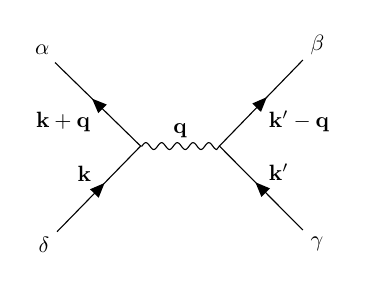
\begin{tikzpicture}[scale=0.8, every node/.style={scale=0.8}]
			  \begin{feynman}
				% Define vertices
				\vertex (a);
				\vertex[below left= 1.5 cm of a] (i1) {$\delta$};
				\vertex[above left =  1.5 cm of a] (f1) {$\alpha$};
				\vertex[right = 1 cm of a] (b);
				\vertex[below right = 1.5 cm of b] (i2) {$\gamma$};
				\vertex[above right= 1.5 cm of b] (f2) {$\beta$};

				% Draw fermion lines
				\diagram*[horizontal'= (a) to (b)] {
				(i1) -- [fermion, edge label=$\mathbf{k}$] (a) -- [fermion, edge label=$ \mathbf{k} + \mathbf{q}$] (f1),
				(i2) -- [fermion, edge label'=$\mathbf{k}'$] (b) -- [fermion, edge label'={$\mathbf{k}'- \mathbf{q}$}] (f2),
				(a) -- [photon, edge label=$\mathbf{q}$] (b),
				};
			\end{feynman}
		  \end{tikzpicture}                                                                                                                                                                                                                                                                \\
		 & = \int \frac{d^{3} r}{V} \int \frac{d^{3} r'}{V} e^{-i \mathbf{q} \cdot (\mathbf{r} - \mathbf{r}')} u_{\alpha \mathbf{k} + \mathbf{q}}^{*}(\mathbf{r}) u_{\beta \mathbf{k'} - \mathbf{q}}^{*}(\mathbf{r}') V_{\text{e-e}} (\mathbf{r} - \mathbf{r}') u_{\gamma \mathbf{k}'}(\mathbf{r}') u_{\delta \mathbf{k}}(\mathbf{r}),
	\end{aligned}
	\label{eq: Coulomb pot}
\end{equation}
trong đó
\begin{gather}
	V_{\text{e-e}}(\mathbf{r} - \mathbf{r}') = \frac{e^{2}}{\epsilon \abs{\mathbf{r} - \mathbf{r}'}}.
\end{gather}
Biến đổi Fourier(thuận) của thế Coulomb
\begin{equation}
	\begin{aligned}
		V_{\text{e-e}}(\mathbf{q})
		 & = \int \frac{d^{3} r}{L^{3}} V_{\text{e-e}}(\mathbf{r}) e^{- i \mathbf{q} \cdot (\mathbf{r})}                                                                                                                                                      \\
		 & = \frac{e^{2}}{\epsilon V} \int \frac{d^{3} r}{\abs{\mathbf{r}}} e^{- i \mathbf{q} \cdot \mathbf{r}} = \frac{e^{2}}{\epsilon V} \int_{0}^{\infty} dr \int_{0}^{\pi} d\theta  \int_{0}^{2\pi} d \phi r \sin \theta e^{- i q r \cos \theta}          \\
		 & = \frac{2 \pi e^{2}}{\epsilon V} \int_{0}^{\infty} r dr \int_{0}^{2\pi} \sin \theta d\theta e^{i q r \cos \theta} = - i \frac{2\pi e^{2}}{ \epsilon V q} \int_{0}^{\infty} dr (e^{iqr} - e^{-iqr})                                                 \\
		 & = - i \frac{2\pi e^{2}}{ \epsilon V q} \lim_{\gamma \to 0} \int_{0}^{\infty} dr (e^{iqr} - e^{-iqr}) e^{-\gamma r}  = \lim\limits_{\gamma \to 0}\frac{4 \pi e^{2}}{\epsilon V} \frac{1}{q^{2} + \gamma^{2}} = \frac{4\pi e^{2}}{\epsilon V q^{2}}.
	\end{aligned}
	\label{eq: FT Coulomb pot}
\end{equation}
Biến đổi Fourier(ngược) của thế Coulomb
\begin{gather}
	V_{\text{e-e}}(\mathbf{r}) = \sum_{\mathbf{q}} V_{\text{e-e}}(\mathbf{q}) e^{i \mathbf{q} \cdot \mathbf{r}}.
	\label{eq: inverse FT Coulomb pot}
\end{gather}
Thay vào \eqref{eq: Coulomb pot}, ta có
\begin{equation}
	\begin{aligned}
		V_{\mathbf{k}, \mathbf{k}', \mathbf{q}}^{\alpha \beta \gamma \delta}
		 & = \int \frac{d^{3} r}{V} \int \frac{d^{3} r'}{V} e^{-i \mathbf{q} \cdot (\mathbf{r} - \mathbf{r}')} u_{\alpha \mathbf{k} + \mathbf{q}}^{*}(\mathbf{r}) u_{\beta \mathbf{k'} - \mathbf{q}}^{*}(\mathbf{r}') \sum_{\mathbf{q}'} V_{\text{e-e}}(\mathbf{q}') e^{i \mathbf{q}' \cdot (\mathbf{r} - \mathbf{r}')} u_{\gamma \mathbf{k}'}(\mathbf{r}') u_{\delta \mathbf{k}}(\mathbf{r}) \\
		 & = \int \frac{d^{3} r}{V} \int \frac{d^{3} r'}{V} \sum_{\mathbf{q}'} V_{\text{e-e}}(\mathbf{q}') e^{i (\mathbf{q}' - \mathbf{q}) \cdot (\mathbf{r} - \mathbf{r}')} u_{\alpha \mathbf{k} + \mathbf{q}}^{*}(\mathbf{r}) u_{\delta \mathbf{k}}(\mathbf{r})  u_{\beta \mathbf{k'} - \mathbf{q}}^{*}(\mathbf{r}') u_{\gamma \mathbf{k}'}(\mathbf{r}') ,
	\end{aligned}
\end{equation}
Đặt $\mathbf{r} \to \mathbf{R}_{i} + \mathbf{r}$, $\mathbf{r}' \to \mathbf{R}_{j} + \mathbf{r}'$ và sử dụng hệ thức $\dps \sum_{i}^{N} e^{i (\mathbf{q}' - \mathbf{q} \cdot \mathbf{R}_{i})} = N \delta_{\mathbf{q}',\mathbf{q}}$, và áp dụng gần đúng sóng dài, phương trình trên trở thành
\begin{equation}
	\begin{aligned}
		V_{\mathbf{k}, \mathbf{k}', \mathbf{q}}^{\alpha \beta \gamma \delta}
		 & \simeq \frac{1}{N^{2}} \sum_{i,j} \sum_{\mathbf{q}'} V_{\text{e-e}}(\mathbf{q}') e^{i ( \mathbf{q}' - \mathbf{q} ) \cdot ( \mathbf{R}_{i} - \mathbf{R}_{j} ) }                                                                                                              \\
		 & \quad \times \int_{V_{\text{cell}}} \frac{d^{3}r}{V} u_{\alpha \mathbf{k} + \mathbf{q}}^{*}(\mathbf{r}) u_{\delta \mathbf{k}}(\mathbf{r}) \int_{V_{\text{cell}}} \frac{d^{3} r'}{V} u_{\beta \mathbf{k'} - \mathbf{q}}^{*}(\mathbf{r}') u_{\gamma \mathbf{k}'}(\mathbf{r}') \\
		 & \simeq V_{\text{e-e}}(\mathbf{q}) \braket{u_{\alpha \mathbf{k} + \mathbf{q}}}{u_{\delta \mathbf{k}}} \braket{u_{\beta \mathbf{k}' - \mathbf{q}}}{u_{\gamma \mathbf{k}'}}.
	\end{aligned}
	\label{eq: matrix elements Coulomb}
\end{equation}
Từ đó ta rút ra phương trình chuyển động Heisenberg với tương tác Coulomb
\begin{equation}
	\begin{aligned}
		 & \frac{d}{dt}  a_{\lambda \mathbf{k}}^{\dagger} a_{\lambda' \mathbf{k}}
		= \frac{i}{\hbar} \langle [ H^{0} + H^{C}, a_{\lambda \mathbf{k}}^{\dagger} a_{\lambda' \mathbf{k}} ] \rangle                                                                                                                                                                                                                                                                                                                                                                                                                      \\
		 & = \frac{i}{\hbar} \langle\left[  \sum_{\nu \mathbf{k}'} \mathcal{E}_{\nu }(\mathbf{k}') a_{\nu \mathbf{k}'}^{\dagger} a_{\nu \mathbf{k}'} + \frac{1}{2} \sum_{\mathbf{k}' \mathbf{k}'' \mathbf{q}} \sum_{\alpha \beta \gamma \delta} V_{\mathbf{k}', \mathbf{k}'', \mathbf{q}}^{\alpha \beta \gamma \delta} a_{\alpha \mathbf{k}'+\mathbf{q}}^{\dagger} a_{\beta \mathbf{k}'' - \mathbf{q}}^{\dagger} a_{\gamma \mathbf{k}''} a_{\delta \mathbf{k}'},  a_{\lambda \mathbf{k}}^{\dagger} a_{\lambda' \mathbf{k}} \right] \rangle \\
		 & = \frac{i}{\hbar} \sum_{\lambda' \mathbf{k}'} \mathcal{E}_{\lambda}(\mathbf{k}') \langle\left[  a_{\lambda' \mathbf{k}'}^{\dagger} a_{\lambda' \mathbf{k}'}, a_{\lambda \mathbf{k}}^{\dagger} a_{\lambda'\mathbf{k}} \right]\rangle \color{red}{\to ( \mathcal{E}_{\lambda}(\mathbf{k}) - \mathcal{E}_{\lambda'}(\mathbf{k}) ) a_{\lambda \mathbf{k}}^{\dagger} a_{\lambda' \mathbf{k}} }                                                                                                                                       \\
		 & \quad \quad \quad \quad + \frac{i}{2\hbar}  \sum_{\mathbf{k}' \mathbf{k}'' \mathbf{q}} \sum_{\alpha \beta \gamma \delta} V_{\mathbf{k}', \mathbf{k}'', \mathbf{q}}^{\alpha \beta \gamma \delta} \langle \left[ a_{\alpha \mathbf{k}'+\mathbf{q}}^{\dagger} a_{\beta \mathbf{k}'' - \mathbf{q}}^{\dagger} a_{\gamma \mathbf{k}''} a_{\delta \mathbf{k}'}, a_{\lambda \mathbf{k}}^{\dagger} a_{\lambda' \mathbf{k}} \right] \rangle                                                                                               \\
		 & = \frac{i}{\hbar} ( \mathcal{E}_{\lambda}(\mathbf{k}) - \mathcal{E}_{\lambda'}(\mathbf{k}) ) \mean{a_{\lambda \mathbf{k}}^{\dagger} a_{\lambda' \mathbf{k}} }                                                                                                                                                                                                                                                                                                                                                                   \\
		 & \quad \quad \quad \quad  + \frac{i}{\hbar} \sum_{\mathbf{k}' \mathbf{q}} \sum_{\alpha \beta \gamma} V_{\mathbf{k}, \mathbf{k}', \mathbf{q}}^{\alpha \beta \gamma \lambda} \mean{a_{\alpha \mathbf{k} + \mathbf{q}}^{\dagger} a_{\beta \mathbf{k}' - \mathbf{q}}^{\dagger} a_{\gamma \mathbf{k}'} a_{\lambda' \mathbf{k}} }                                                                                                                                                                                                      \\
		 & \quad \quad \quad \quad + \frac{i}{\hbar} \sum_{\mathbf{k}' \mathbf{q}} \sum_{\alpha \gamma \delta} V_{\mathbf{k}', \mathbf{k} + \mathbf{q}, \mathbf{q}}^{\alpha \lambda' \gamma \delta} \mean{a_{\lambda \mathbf{k}}^{\dagger} a_{\alpha \mathbf{k}' + \mathbf{q}}^{\dagger} a_{\gamma \mathbf{k} + \mathbf{q}} a_{\delta'} },                                                                                                                                                                                       \\
	\end{aligned}
	\label{eq: equation of motion with Coulomb}
\end{equation}
chú ý
\begin{equation*}
	\begin{aligned}
		& \frac{i}{2\hbar}  \sum_{\mathbf{k}' \mathbf{k}'' \mathbf{q}} \sum_{\alpha \beta \gamma \delta} V_{\mathbf{k}', \mathbf{k}'', \mathbf{q}}^{\alpha \beta \gamma \delta} \left[ a_{\alpha \mathbf{k}'+\mathbf{q}}^{\dagger} a_{\beta \mathbf{k}'' - \mathbf{q}}^{\dagger} a_{\gamma \mathbf{k}''} a_{\delta \mathbf{k}'}, a_{\lambda \mathbf{k}}^{\dagger} a_{\lambda' \mathbf{k}} \right] \\
		&= \frac{i}{2\hbar}  \sum_{\mathbf{k}' \mathbf{k}'' \mathbf{q}} \sum_{\alpha \beta \gamma \delta} V_{\mathbf{k}', \mathbf{k}'', \mathbf{q}}^{\alpha \beta \gamma \delta} \left( a_{\alpha \mathbf{k}'+\mathbf{q}}^{\dagger} a_{\beta \mathbf{k}'' - \mathbf{q}}^{\dagger} a_{\gamma \mathbf{k}''} a_{\delta \mathbf{k}'} a_{\lambda \mathbf{k}}^{\dagger} a_{\lambda' \mathbf{k}} - a_{\lambda \mathbf{k}} ^{\dagger} a_{\lambda' \mathbf{k}} a_{\alpha \mathbf{k}'+\mathbf{q}}^{\dagger} a_{\beta\mathbf{k}''-\mathbf{q}}^{\dagger} a_{\gamma \mathbf{k}''} a_{\delta \mathbf{k}'} \right) \\
		& = \frac{i}{2\hbar}  \sum_{\mathbf{k}' \mathbf{k}'' \mathbf{q}} \sum_{\alpha \beta \gamma \delta} V_{\mathbf{k}', \mathbf{k}'', \mathbf{q}}^{\alpha \beta \gamma \delta} \bigg( a_{\alpha \mathbf{k}' + \mathbf{q}}^{\dagger} a_{\beta \mathbf{k}'' - \mathbf{q}}^{\dagger} a_{\gamma \mathbf{k}''} (\delta_{\delta \lambda} \delta_{\mathbf{k}', \mathbf{k}} - a_{\lambda \mathbf{k}}^{\dagger} a_{\delta \mathbf{k}'}) a_{\lambda' \mathbf{k}}   \\
		& \quad - a_{\lambda \mathbf{k}}^{\dagger} ( \delta_{\lambda' \alpha} \delta_{\mathbf{k}, \mathbf{k}' + \mathbf{q}} - a_{\alpha \mathbf{k}'+ \mathbf{q}}^{\dagger} a_{\lambda' \mathbf{k}} ) a_{\beta\mathbf{k}''-\mathbf{q}}^{\dagger} a_{\gamma \mathbf{k}''} a_{\delta \mathbf{k}'} \bigg) \\
		& = \frac{i}{2\hbar}  \sum_{\mathbf{k}' \mathbf{k}'' \mathbf{q}} \sum_{\alpha \beta \gamma \delta} V_{\mathbf{k}', \mathbf{k}'', \mathbf{q}}^{\alpha \beta \gamma \delta} \bigg( a_{\alpha \mathbf{k}' + \mathbf{q}}^{\dagger} a_{\beta \mathbf{k}'' - \mathbf{q}}^{\dagger} a_{\gamma \mathbf{k}''} \delta_{\delta \lambda} \delta_{\mathbf{k}', \mathbf{k}} a_{\lambda' \mathbf{k}} -  a_{\alpha \mathbf{k}' + \mathbf{q}}^{\dagger} a_{\beta \mathbf{k}''  - \mathbf{q}}^{\dagger} a_{\gamma \mathbf{k}''} a_{\lambda \mathbf{k}}^{\dagger} a_{\delta \mathbf{k}'} a_{\lambda' \mathbf{k}}  \\
		& \quad - a_{\lambda \mathbf{k}}^{\dagger} \delta_{\lambda' \alpha} \delta_{\mathbf{k}, \mathbf{k}' + \mathbf{q}} a_{\beta\mathbf{k}''-\mathbf{q}}^{\dagger} a_{\gamma \mathbf{k}''} a_{\delta \mathbf{k}'} + a_{\lambda \mathbf{k}}^{\dagger} a_{\alpha \mathbf{k}'+ \mathbf{q}}^{\dagger} a_{\lambda' \mathbf{k}} a_{\beta\mathbf{k}''-\mathbf{q}}^{\dagger} a_{\gamma \mathbf{k}''} a_{\delta \mathbf{k}'} \bigg) \\
		& =  \frac{i}{2\hbar}  \sum_{\mathbf{k}' \mathbf{k}'' \mathbf{q}} \sum_{\alpha \beta \gamma \delta} V_{\mathbf{k}', \mathbf{k}'', \mathbf{q}}^{\alpha \beta \gamma \delta} \bigg( a_{\alpha \mathbf{k}' + \mathbf{q}}^{\dagger} a_{\beta \mathbf{k}'' - \mathbf{q}}^{\dagger} a_{\gamma \mathbf{k}''} \delta_{\delta \lambda} \delta_{\mathbf{k}', \mathbf{k}} a_{\lambda' \mathbf{k}} - a_{\alpha \mathbf{k}' + \mathbf{q}}^{\dagger} a_{\beta \mathbf{k}'' - \mathbf{q}}^{\dagger} ( \delta_{\gamma \lambda} \delta_{\mathbf{k}'', \mathbf{k}} - a_{\lambda \mathbf{k}}^{\dagger} a_{\gamma \mathbf{k}''} ) a_{\delta \mathbf{k}'} a_{\lambda' \mathbf{k}} \\
		& \quad - a_{\lambda \mathbf{k}}^{\dagger} \delta_{\lambda' \alpha} \delta_{\mathbf{k}, \mathbf{k}' + \mathbf{q}} a_{\beta\mathbf{k}''-\mathbf{q}}^{\dagger} a_{\gamma \mathbf{k}''} a_{\delta \mathbf{k}'} + a_{\lambda \mathbf{k}}^{\dagger} a_{\alpha \mathbf{k}' + \mathbf{q}}^{\dagger} ( \delta_{\lambda' \beta} \delta_{\mathbf{k}, \mathbf{k}'' - \mathbf{q}} - a_{\beta \mathbf{k}'' - \mathbf{q}}^{\dagger} a_{\lambda' \mathbf{k}} ) a_{\gamma \mathbf{k}''} a_{\delta \mathbf{k}'} \bigg)\\
		& =  \frac{i}{2\hbar}  \sum_{\mathbf{k}' \mathbf{k}'' \mathbf{q}} \sum_{\alpha \beta \gamma \delta} V_{\mathbf{k}', \mathbf{k}'', \mathbf{q}}^{\alpha \beta \gamma \delta} \bigg( a_{\alpha \mathbf{k}' + \mathbf{q}}^{\dagger} a_{\beta \mathbf{k}'' - \mathbf{q}}^{\dagger} a_{\gamma \mathbf{k}''} \delta_{\delta \lambda} \delta_{\mathbf{k}', \mathbf{k}} a_{\lambda' \mathbf{k}} - a_{\alpha \mathbf{k}' + \mathbf{q}}^{\dagger} a_{\beta \mathbf{k}'' - \mathbf{q}}^{\dagger} \delta_{\gamma \lambda} \delta_{\mathbf{k}'', \mathbf{k}} a_{\delta \mathbf{k}'} a_{\lambda' \mathbf{k}} \\
		& \quad + \cancel{ a_{\alpha \mathbf{k}' + \mathbf{q}}^{\dagger} a_{\beta \mathbf{k}'' - \mathbf{q}}^{\dagger} a_{\lambda \mathbf{k}}^{\dagger} a_{\gamma \mathbf{k}''} a_{\delta \mathbf{k}'} a_{\lambda' \mathbf{k}} } - a_{\lambda \mathbf{k}}^{\dagger} \delta_{\lambda' \alpha} \delta_{\mathbf{k}, \mathbf{k}' + \mathbf{q}} a_{\beta\mathbf{k}''-\mathbf{q}}^{\dagger} a_{\gamma \mathbf{k}''} a_{\delta \mathbf{k}'} \\
		& \quad + a_{\lambda \mathbf{k}}^{\dagger} a_{\alpha \mathbf{k}' + \mathbf{q}}^{\dagger} \delta_{\lambda' \beta} \delta_{\mathbf{k}, \mathbf{k}'' - \mathbf{q}} a_{\gamma \mathbf{k}''} a_{\delta \mathbf{k}'} - \cancel{a_{\lambda \mathbf{k}}^{\dagger} a_{\alpha \mathbf{k}' + \mathbf{q}}^{\dagger}  a_{\beta \mathbf{k}'' - \mathbf{q}}^{\dagger} a_{\lambda' \mathbf{k}} a_{\gamma \mathbf{k}''} a_{\delta \mathbf{k}'}} \bigg) \\
		& = \frac{i}{2\hbar} \sum_{\mathbf{k}'' \mathbf{q}} \sum_{\alpha \beta \gamma} V_{\mathbf{k}, \mathbf{k}'', \mathbf{q}}^{\alpha \beta \gamma \lambda} a_{\alpha \mathbf{k} + \mathbf{q}}^{\dagger} a_{\beta \mathbf{k}'' - \mathbf{q}}^{\dagger} a_{\gamma \mathbf{k}''} a_{\lambda' \mathbf{k}} - \underbracket{ \frac{i}{2\hbar} \sum_{\mathbf{k}' \mathbf{q}} \sum_{\alpha \beta \delta} V_{\mathbf{k}', \mathbf{k}, \mathbf{q}}^{\alpha \beta \lambda \delta} \overbracket{a_{\alpha \mathbf{k}' + \mathbf{q}}^{\dagger} a_{\beta \mathbf{k} - \mathbf{q}}^{\dagger}}^{ = - a_{\beta \mathbf{k} - \mathbf{q}}^{\dagger} a_{\alpha \mathbf{k}' + \mathbf{q}}^{\dagger} } a_{\delta \mathbf{k}'} a_{\lambda' \mathbf{k}} }_{ \mathbf{q} \to - \mathbf{q}, \alpha \leftrightarrow \beta, \delta \to \gamma, V_{-\mathbf{q}} = V_{\mathbf{q}} } \\
		& \quad - \underbracket{ \frac{i}{2\hbar} \sum_{\mathbf{k}'' \mathbf{q}} \sum_{\beta \gamma \delta} V_{\mathbf{k} - \mathbf{q}, \mathbf{k}'', \mathbf{q}}^{\lambda' \beta \gamma \delta} a_{\lambda \mathbf{k}}^{\dagger} a_{\beta \mathbf{k}'' - \mathbf{q}}^{\dagger} \overbracket{a_{\gamma \mathbf{k}''} a_{\delta \mathbf{k} - \mathbf{q}}}^{ = - a_{\delta \mathbf{k} - \mathbf{q}} a_{\gamma \mathbf{k}''} } }_{ \mathbf{q} \to - \mathbf{q}, \delta \leftrightarrow \gamma, \beta \to \alpha, V_{-\mathbf{q}} = V_{\mathbf{q}} } + \frac{i}{2\hbar} \sum_{\mathbf{k}' \mathbf{q}} \sum_{\alpha \gamma \delta} V_{\mathbf{k}', \mathbf{k} + \mathbf{q}, \mathbf{q}}^{\alpha \lambda' \gamma \delta} a_{\lambda \mathbf{k}}^{\dagger} a_{\alpha \mathbf{k}' + \mathbf{q}}^{\dagger} a_{\gamma \mathbf{k} + \mathbf{q}} a_{\delta \mathbf{k}'} \\
		& = \frac{i}{2\hbar} \sum_{\mathbf{k}'' \mathbf{q}} \sum_{\alpha \beta \gamma} V_{\mathbf{k}, \mathbf{k}'', \mathbf{q}}^{\alpha \beta \gamma \lambda} a_{\alpha \mathbf{k} + \mathbf{q}}^{\dagger} a_{\beta \mathbf{k}'' - \mathbf{q}}^{\dagger} a_{\gamma \mathbf{k}''} a_{\lambda' \mathbf{k}} + \frac{i}{2\hbar} \sum_{\mathbf{k}' \mathbf{q}} \sum_{ \alpha \beta \gamma } V_{\mathbf{k}', \mathbf{k}, \mathbf{q}}^{\alpha \beta \lambda \gamma} a_{\alpha \mathbf{k} + \mathbf{q}}^{\dagger} a_{\beta \mathbf{k}' - \mathbf{q}}^{\dagger} a_{ \gamma \mathbf{k}' } a_{\lambda' \mathbf{k}} \\
		& + \quad \frac{i}{2\hbar} \sum_{\mathbf{k}'' \mathbf{q}} \sum_{\alpha \gamma \delta} V_{\mathbf{k}', \mathbf{k} + \mathbf{q}, \mathbf{q}}^{\lambda' \alpha \gamma \delta} a_{\lambda \mathbf{k}}^{\dagger} a_{\alpha \mathbf{k}'' + \mathbf{q}}^{\dagger} a_{\gamma \mathbf{k}''} a_{\delta \mathbf{k} + \mathbf{q}} + \frac{i}{2\hbar} \sum_{\mathbf{k}' \mathbf{q}} \sum_{\alpha \gamma \delta} V_{\mathbf{k}', \mathbf{k} + \mathbf{q}, \mathbf{q}}^{\alpha \lambda' \gamma \delta} a_{\lambda \mathbf{k}}^{\dagger} a_{\alpha \mathbf{k}' + \mathbf{q}}^{\dagger} a_{\gamma \mathbf{k}'} a_{\delta \mathbf{k} + \mathbf{q}}.
	\end{aligned}
\end{equation*}
Phương trình \eqref{eq: equation of motion with Coulomb} là phương trình không đóng. Vì thế, ta cần áp dụng gần đúng giá trị trung bình của 4 toán tử trong phương trình \eqref{eq: equation of motion with Coulomb} bằng tích của 2 giá trị trung bình của 2 toán tử(gần đúng Hartree-Fock), sao cho có được cặp toán tử liên quan
\begin{equation}
	\begin{aligned}
		\mean{ a_{\alpha \mathbf{k} + \mathbf{q}}^{\dagger} a_{\beta \mathbf{k}' - \mathbf{q}}^{\dagger} a_{\gamma \mathbf{k}'} a_{\lambda' \mathbf{k}} } &\simeq - \mean{a_{\alpha \mathbf{k} + \mathbf{q}}^{\dagger} a_{\gamma \mathbf{k} + \mathbf{q}} } \mean{ a_{\beta \mathbf{k}}^{\dagger} a_{\lambda' \mathbf{k}} } \delta_{\mathbf{k}' + \mathbf{k} + \mathbf{q}}, \\
		\mean{a_{\lambda \mathbf{k}}^{\dagger} a_{\alpha \mathbf{k}' + \mathbf{q}}^{\dagger} a_{\gamma \mathbf{k} + \mathbf{q}} a_{\delta'} } & \simeq \mean{ a_{\alpha \mathbf{k} + \mathbf{q}}^{\dagger} a_{\gamma \mathbf{k} + \mathbf{q}} } \mean{ a_{\lambda \mathbf{k}}^{\dagger} a_{\delta \mathbf{k}} } \delta_{\mathbf{k}, \mathbf{k}'}.
	\end{aligned}
\end{equation}
Thay phương trình trên vào \eqref{eq: equation of motion with Coulomb}, ta được
\begin{equation}
	\begin{aligned}
		\frac{d}{dt} \mean{ a_{\lambda \mathbf{k}}^{\dagger} a_{\lambda' \mathbf{k}} } 
		& = \frac{i}{\hbar} ( \mathcal{E}_{\lambda}(\mathbf{k}) - \mathcal{E}_{\lambda'}(\mathbf{k}) ) \mean{a_{\lambda \mathbf{k}}^{\dagger} a_{\lambda' \mathbf{k}} } \\
		& \quad \underbracket{- \frac{i}{\hbar} \sum_{\mathbf{q}} \sum_{\alpha \beta \gamma} V_{\mathbf{k}, \mathbf{k} + \mathbf{q}, \mathbf{q}}^{\alpha \beta \gamma \lambda} \mean{a_{\alpha \mathbf{k} + \mathbf{q}}^{\dagger} a_{\gamma \mathbf{k} + \mathbf{q}} } \mean{ a_{\beta \mathbf{k}}^{\dagger} a_{\lambda' \mathbf{k}} }}_{ \beta \to \gamma, \gamma \to \mu } \\
		& \quad  \underbracket{+ \frac{i}{\hbar} \sum_{\mathbf{q}} \sum_{\alpha \gamma \delta} V_{\mathbf{k}, \mathbf{k} + \mathbf{q}, \mathbf{q}}^{\alpha \lambda' \gamma \delta} \mean{ a_{\alpha \mathbf{k} + \mathbf{q}}^{\dagger} a_{\gamma \mathbf{k} + \mathbf{q}} } \mean{ a_{\lambda \mathbf{k}}^{\dagger} a_{\delta \mathbf{k}} }}_{\gamma \to \beta, \delta \to \mu} \\ 
		& = \frac{i}{\hbar} ( \mathcal{E}_{\lambda}(\mathbf{k}) - \mathcal{E}_{\lambda'}(\mathbf{k}) ) \mean{a_{\lambda \mathbf{k}}^{\dagger} a_{\lambda' \mathbf{k}} } \\
		& \quad - \frac{i}{\hbar} \sum_{\mathbf{q}} \sum_{\alpha \mu \beta} V_{\mathbf{k}, \mathbf{k} + \mathbf{q}, \mathbf{q}}^{\alpha \mu \beta \lambda} \mean{ a_{\alpha \mathbf{k} + \mathbf{q}}^{\dagger} a_{\beta \mathbf{k} + \mathbf{q}} } \mean{ a_{\mu \mathbf{k}}^{\dagger} a_{\lambda' \mathbf{k}} } \\
		& \quad + \frac{i}{\hbar} \sum_{\mathbf{q}} \sum_{\alpha \beta \mu} V_{\mathbf{k}, \mathbf{k} + \mathbf{q}, \mathbf{q}}^{\alpha \lambda' \beta \mu} \mean{ a_{\alpha \mathbf{k} + \mathbf{q}}^{\dagger} a_{\beta \mathbf{k} + \mathbf{q}} } \mean{ a_{\lambda \mathbf{k}}^{\dagger} a_{\mu \mathbf{k}} } \\
		& = \frac{i}{\hbar} ( \mathcal{E}_{\lambda}(\mathbf{k}) - \mathcal{E}_{\lambda'}(\mathbf{k}) ) \mean{a_{\lambda \mathbf{k}}^{\dagger} a_{\lambda' \mathbf{k}} } \\
		& \quad - \frac{i}{\hbar} \sum_{\mu} \left[ \Sigma_{\mu \lambda}(\mathbf{k}) \mean{ a_{\mu \mathbf{k}}^{\dagger} a_{\lambda' \mathbf{k}} } - \Sigma_{\lambda' \mu}(\mathbf{k}) \mean{ a_{\lambda \mathbf{k}}^{\dagger} a_{\mu \mathbf{k}} } \right],
	\end{aligned}
\end{equation}
trong đó 
\begin{equation}
	\begin{aligned}
		\Sigma_{\mu \lambda}(\mathbf{k}) = \sum_{\alpha \beta \mathbf{q}} V_{\mathbf{k}, \mathbf{k} + \mathbf{q}, \mathbf{q}}^{\alpha \mu \beta \lambda} \mean{ a_{\alpha \mathbf{k} + \mathbf{q}}^{\dagger} a_{\beta \mathbf{k} + \mathbf{q}} }, \\
		\Sigma_{\lambda' \mu}(\mathbf{k}) = \sum_{\alpha \beta \mathbf{q}} V_{\mathbf{k}, \mathbf{k} + \mathbf{q}, \mathbf{q}}^{\alpha \lambda' \beta \mu} \mean{ a_{\alpha \mathbf{k} + \mathbf{q}}^{\dagger} a_{\beta \mathbf{k} + \mathbf{q}} }.
	\end{aligned}
\end{equation}
Sử dụng định nghĩa \eqref{eq: operator charge density matrix elements reduced}, ta có được phương trình chuyển động trong gần đúng Hartree-Fock có tương tác Coulomb
\begin{equation}
	\begin{aligned}
		\frac{d}{dt} \rho_{\lambda \lambda'}(\mathbf{k})
		& = - \frac{i}{\hbar} ( \mathcal{E}_{\lambda}(\mathbf{k}) - \mathcal{E}_{\lambda'}(\mathbf{k}) ) \rho_{\lambda \lambda'}(\mathbf{k}) \\
		& \quad + \frac{i}{\hbar} \sum_{\mu} \left[ \Sigma_{\lambda \mu}(\mathbf{k}) \rho_{\mu \lambda'}(\mathbf{k}) - \rho_{\lambda \mu} \Sigma_{\mu \lambda'}(\mathbf{k})  \right],
	\end{aligned}
	\label{eq: equation of motion in HF with Coulomb}
\end{equation}
trong đó 
\begin{equation}
	\begin{aligned}
		\Sigma_{\mu \lambda}(\mathbf{k}) = \sum_{\alpha \beta \mathbf{q}} V_{\mathbf{k}, \mathbf{k} + \mathbf{q}, \mathbf{q}}^{\alpha \mu \beta \lambda} \rho_{\mathbf{k} + \mathbf{q}}^{\beta \alpha}, \\
		\Sigma_{\lambda' \mu}(\mathbf{k}) = \sum_{\alpha \beta \mathbf{q}} V_{\mathbf{k}, \mathbf{k} + \mathbf{q}, \mathbf{q}}^{\alpha \lambda' \beta \mu} \rho_{\mathbf{k} + \mathbf{q}}^{\beta \alpha},
	\end{aligned}
\end{equation}
là năng lượng riêng trao đổi.

Kết hợp phương trình \eqref{eq: equation of motion in HF with Coulomb} vào phương trình \eqref{eq: equation of motion in LG} ta được phương trình Bloch bán dẫn có tương tác ánh sáng và tương tác Coulomb trong gauge độ dài là
\begin{equation}
	\begin{aligned}
		\frac{d}{dt} \rho_{\lambda \lambda'}(\mathbf{k})
		& = - \frac{i}{\hbar} ( \mathcal{E}_{\lambda}(\mathbf{k}) - \mathcal{E}_{\lambda'}(\mathbf{k}) ) \rho_{\lambda \lambda'}(\mathbf{k}) \\
		& \quad + \frac{i}{\hbar} \sum_{\mu} \left[ \Sigma_{\lambda \mu}(\mathbf{k}) \rho_{\mu \lambda'}(\mathbf{k}) - \rho_{\lambda \mu} \Sigma_{\mu \lambda'}(\mathbf{k})  \right] \\
		& - \frac{ie}{\hbar} \mathbf{E}(t) \cdot \sum_{ \mu } \left( \boldsymbol{\xi}_{\lambda \mu}(\mathbf{k}) \rho_{\mu \lambda'}(\mathbf{k}) - \rho_{\lambda \mu}(\mathbf{k}) \boldsymbol{\xi}_{\mu \lambda'}(\mathbf{k})\right) + \frac{e}{\hbar} \mathbf{E}(t) \cdot \nabla_{\mathbf{k}} \rho_{\lambda \lambda'}(\mathbf{k}) \\
		& =  - \frac{i}{\hbar} ( \mathcal{E}_{\lambda}(\mathbf{k}) - \mathcal{E}_{\lambda'}(\mathbf{k}) ) \rho_{\lambda \lambda'}(\mathbf{k}) \\
		& \quad - i \sum_{\mu} \left( \Omega_{\lambda \mu}(\mathbf{k}) \rho_{\mu \lambda'}(\mathbf{k}) - \rho_{\lambda \mu}(\mathbf{k}) \Omega_{\mu \lambda'}(\mathbf{k}) \right) + \frac{e}{\hbar} \mathbf{E}(t) \cdot \nabla_{\mathbf{k}} \rho_{\lambda \lambda'}(\mathbf{k}) .
	\end{aligned}
	\label{eq: equation of motion in HF general}
\end{equation} 
\section{Hamiltonian tight-binding 3 bands}
\subsection{Tương tác Coulomb}
\begin{equation}
	\begin{aligned}
		V_{\lambda_{1} \lambda_{2} \lambda_{3} \lambda_{4}} (\mathbf{k}, \mathbf{k}', \mathbf{k}' - \mathbf{k})
		& = \frac{e^{2}}{2 \varepsilon \varepsilon_{0} L^{2}} \frac{1}{\abs{\mathbf{k}' - \mathbf{k}}} \sum_{j} C_{j}^{\lambda_{1}*}(\mathbf{k}') C_{j}^{\lambda_{4}}(\mathbf{k}) \sum_{j'} C_{j'}^{\lambda_{2}*}(\mathbf{k}) C_{j'}^{\lambda_{3}}(\mathbf{k}') \\
		& = 
	\end{aligned}
\end{equation}



\end{document}
